The Compact Muon Solenoid (CMS) detector operates at the LHC at CERN. It was designed to operate in proton-proton (and lead-lead)
collisions at a center-of-mass energy of 14\TeV (5.5\TeV) and at
luminosities up to 10$^{34}$cm$^{-2}$s$^{-1}$
(10$^{27}$cm$^{-2}$s$^{-1}$). The CMS has cilindrical geometry and
its dimensions are a length of 21.5 m, a diameter of 14.6, and a total
weight of 12,500 tons. At the heart of the CMS detector system
lies a 4\unit{T} magnetic field produced by a large-bore superconducting
solenoid which encloses a silicon -- pixel and strips -- tracker, a homogeneous
lead-tungstate crystal electromagnetic calorimeter, and a brass-scintillator
sampling hadron calorimeter. Outside the superconducting solenoid lies
an iron yoke for magnetic flux-return instrumented with four stations
for muon detection. Forward sampling calorimeters extend the rapidity
coverage up to $\eta < 5$ and thus ensure good
hemiticity. Figure~\ref{fig:cmsDetector} shows an schematic representation
of the CMS detector and Figure~\ref{fig:cmsSlice} shows a cartoon
with a cross-sectional-slice view of the CMS detector along with
different particle detections.
\begin{figure}
 \centering
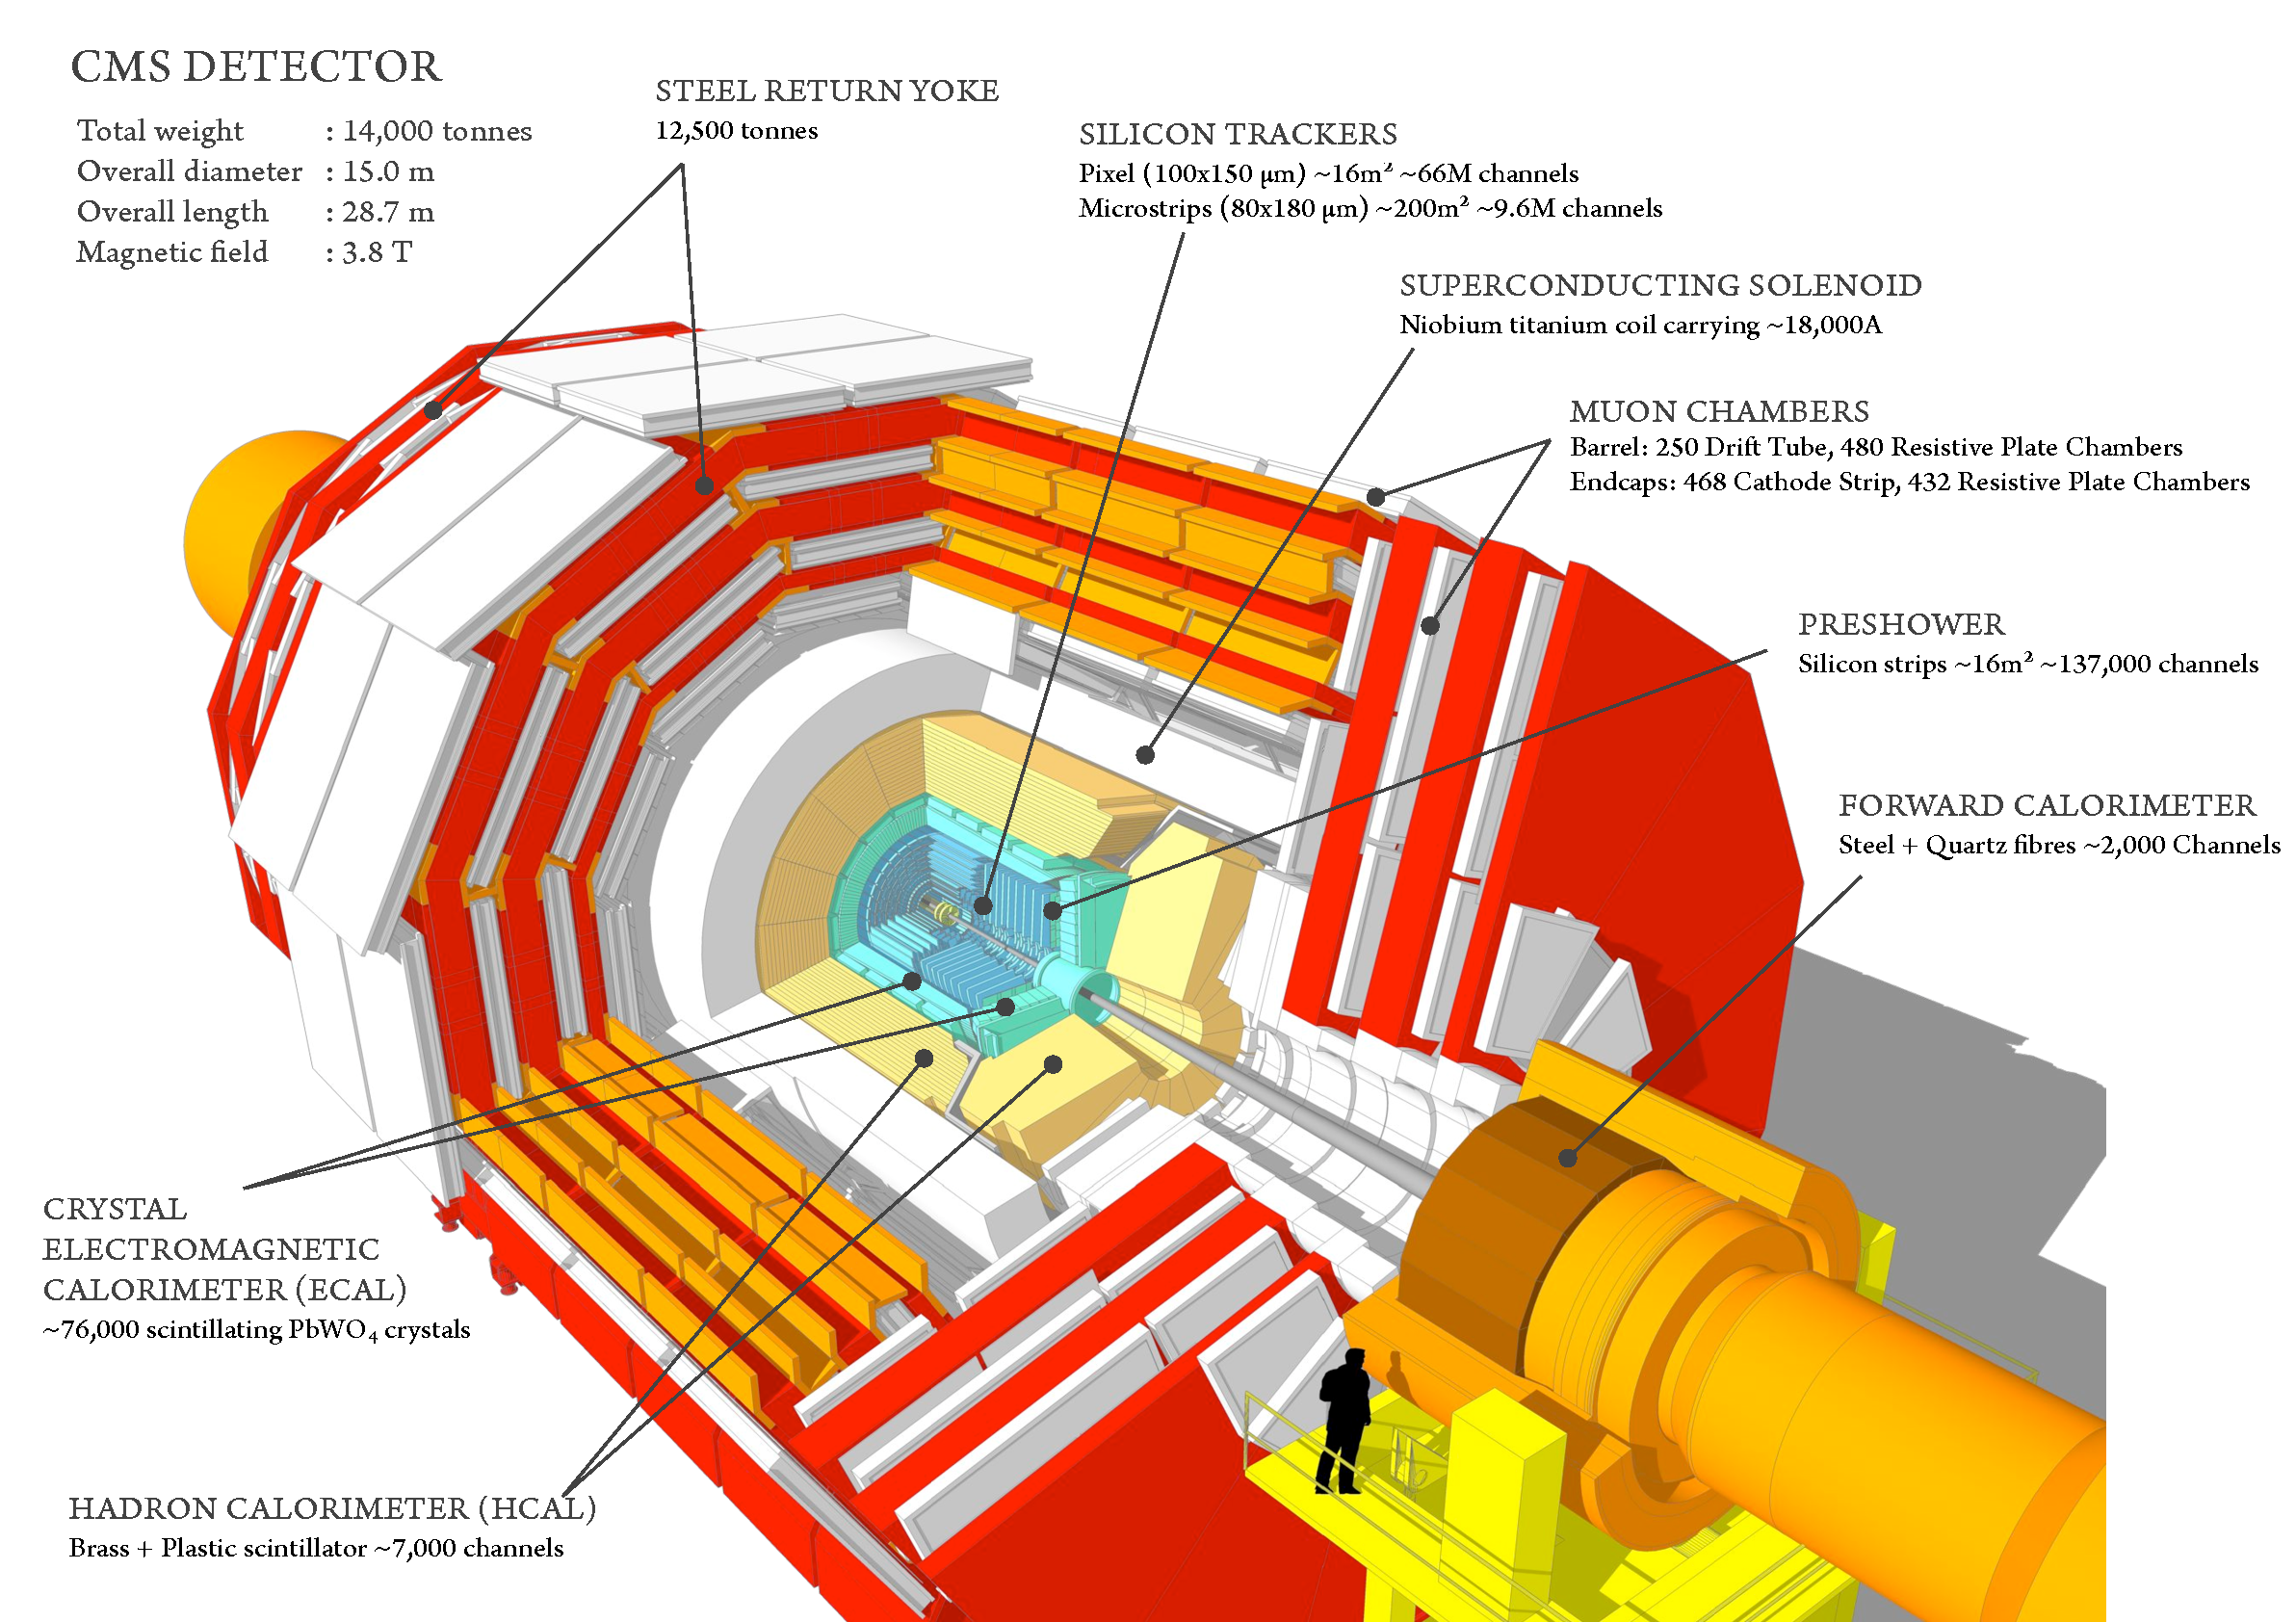
\includegraphics[width=0.99\textwidth]{CMS_DetectorFigures/cms_detector.png}
 \caption{A perspective view of the CMS detector.\label{fig:cmsDetector}}
\end{figure}
\begin{figure}
 \centering
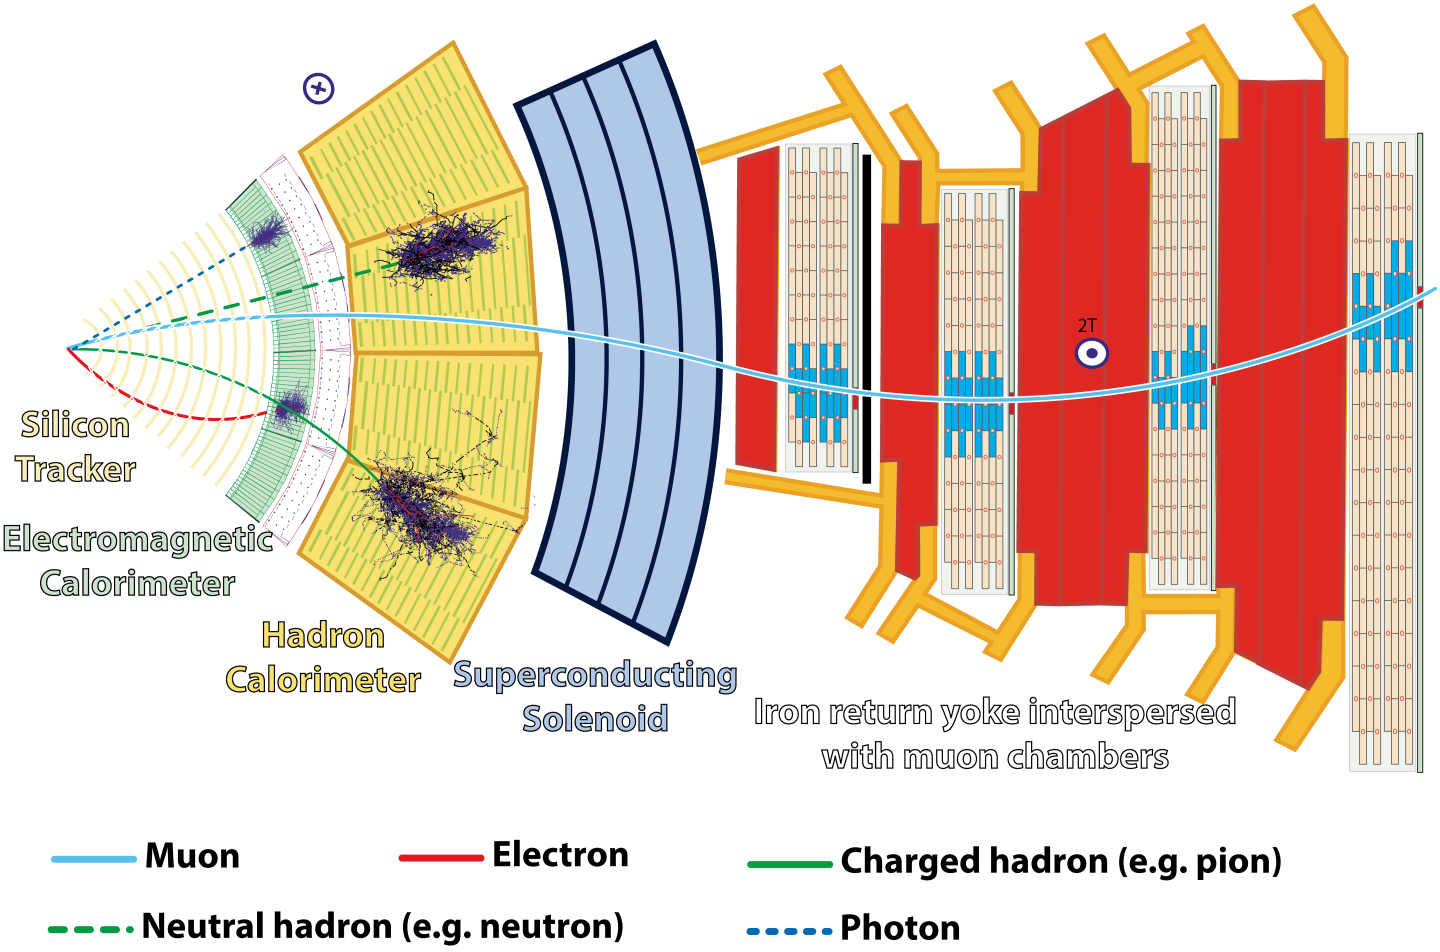
\includegraphics[width=0.99\textwidth]{CMS_DetectorFigures/CMSslice.png}
 \caption{A cross-sectional-slice view of the CMS detector. The
   different components of the detector are clearly labeled and
   different particle detections are depicted.\label{fig:cmsSlice}}
\end{figure}

This chapter presents an introduction to the CMS detector systems and
reconstruction algorithms. It is by no means a complete picture of the
CMS detector and its mostly based on Ref.~\cite{Chatrchyan:2008zzk}.
\section{The Tracker System}
The tracker is the innermost system of the CMS detector.
It was designed to measure efficiently and precisely the trajectories
of charged particles coming from the interaction points, as well as to
provide a precise reconstruction of the secondary vertices at each
bunch crossing. When running at the LHC designed conditions, every
buch crossing, i.e 25 ns, the number of proton-proton collision will
be about 20 and they will produce an average number of particles of about
1000. These conditions and the above requirements implied a highly granular and fast
response design. That being said, this design due to its high power
consumption requires an efficient cooling system which in turn is in
conflict with the goal of minimizing the material budget and thus
reduce unwanted interactions. In addition, the harsh radiation
environment that will deteriorate the detector performance posed
further challenges in its construction. Therefore, the system --
silicon sensors, readout, mechanical structures, granularity, etc --
was designed to operate for 10 year and satisfying the considerations
listed above. The CMS tracker is composed of three layers of pixels
detectors up to a radius of 10.2 cm, a 10-layer silicon strip tracker
up to a radious of 1.1 m, two endcap disks at each side of the barrel pixel detectors, 3
endcap disks at each side of the inner region of the strips (up to a
radius of 55 cm), and finally 9 disks covering the $|z|$ > 120 cm
regions starting a radious of 55 cm. More details about the tracker
layout will be given below and are summarized in
Figure~\ref{fig:trackerlayout}. The tracker covers up to
pseudorapidities of $|eta| < 2.5$ with a about 200 m$^2$ of active
silicon area implemented. The material budget of the CMS tracker is
shown in Figure~\ref{fig:materialBudget}. As it can be seen the most
heavily implemented pseudorapidity is found to be at $|\eta|\approx$ 1.4.
\begin{figure}
 \centering
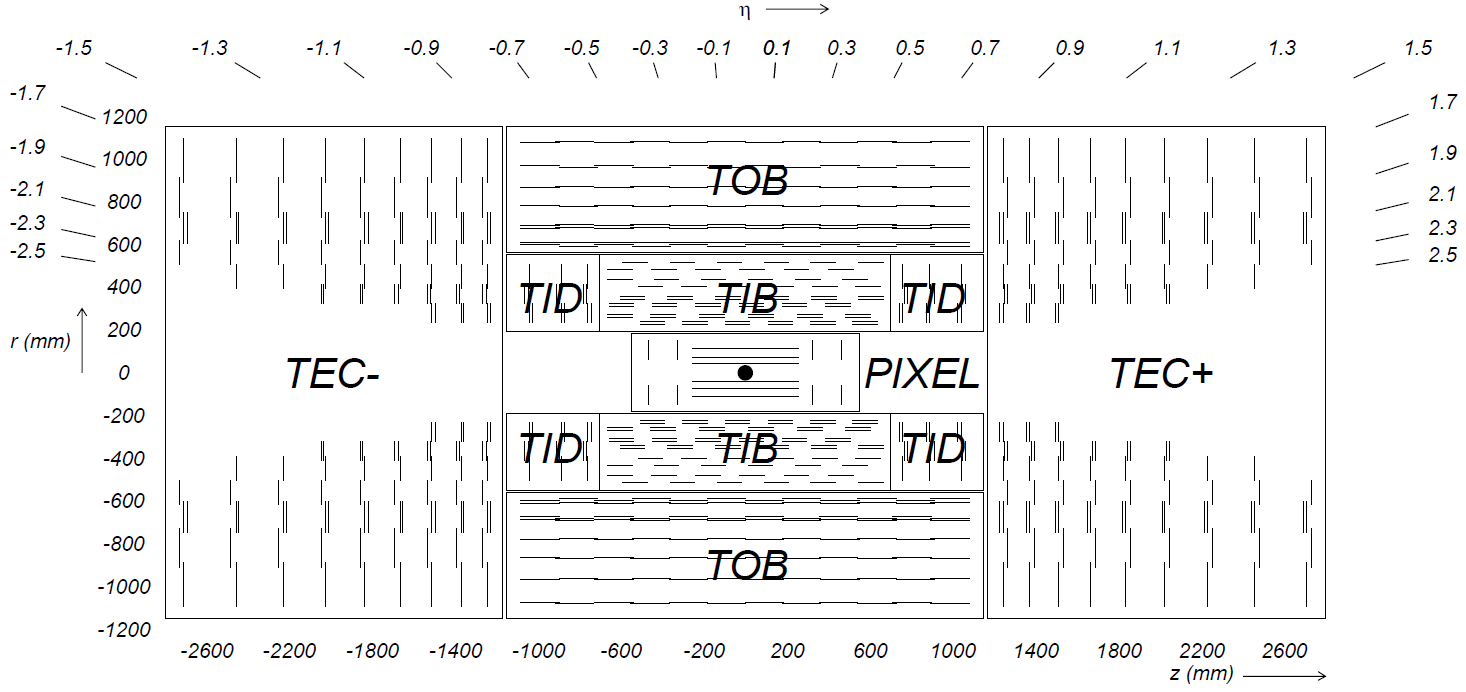
\includegraphics[width=0.99\textwidth]{CMS_DetectorFigures/TrackerLayout.png}
 \caption{A cross-sectional view of the silicon tracker layout. The
   different subsytems are clearly labeled.\label{fig:trackerlayout}}
\end{figure}
\begin{figure}
 \centering
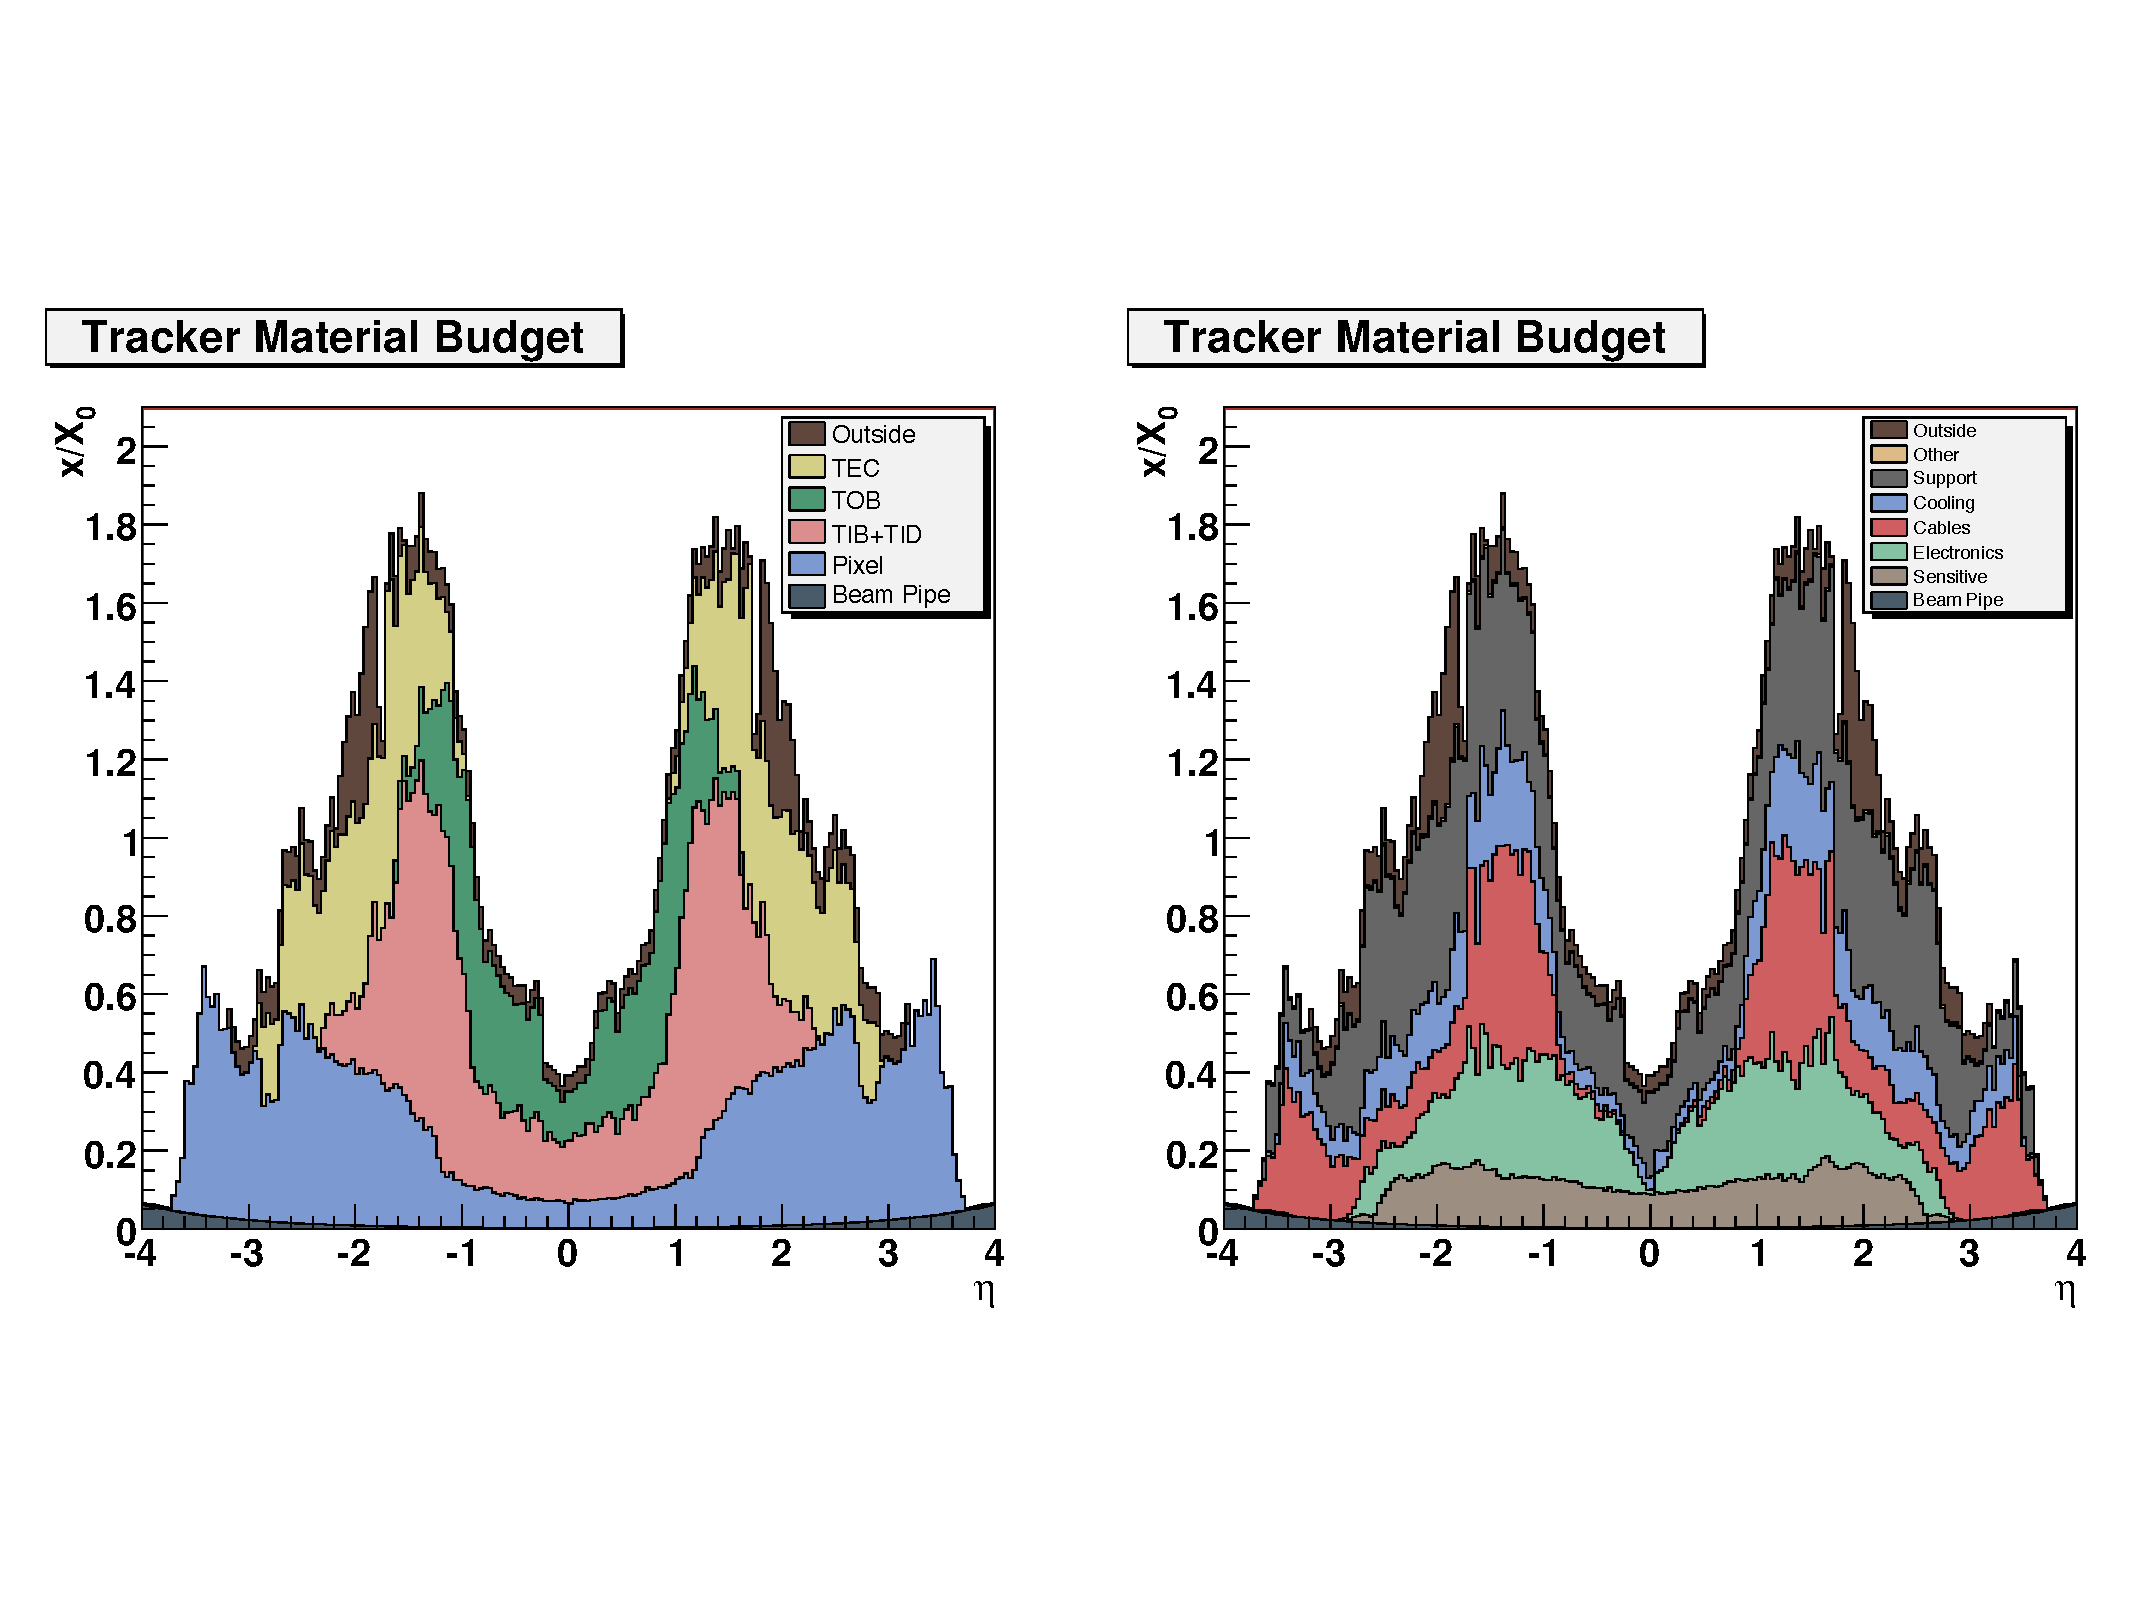
\includegraphics[width=0.99\textwidth]{CMS_DetectorFigures/TrackerMaterialBudget.pdf}
 \caption{Material budget of the CMS tracker in units of radiation
   length as a function of pseudorapidity $\eta$ for the (left)
   different subdetectors and (right) functional contributions.\label{fig:materialBudget}}
\end{figure}
\subsection{Pixel Tracker}
The inner pixel detector is composed of three 53-cm-long cylindrical layers at a
radii of 4.4, 7.3, and 10.2 cm -- which is called BPix. It is finalized by two disks of pixel
modules at each side extending from approximately 6 to 15 cm in
radius -- which is called FPix. The barrel is composed of 672 full and 96 half modules, a full (half)
module is composed of 16 (8) read-out chips equipped with 52$\times$80 pixels
of size 100$\times$150 $\mu$m. A completed full-module has the
dimensions of 66 mm$\times$26 mm and is provided with readout and
power. Figure~\ref{fig:Bpix} shows a completed full- and half- module as
well as an schematic of the different component integrated in the
module. The two disks at each side of the pixel barrel (see
Figure~\ref{fig:trackerlayout}) is composed 24 modules -- with a
trapezoidal geometry. Each disk is composed of two different
panel types; the first and closest to the interaction point is formed
by a 1$\times$2, 2$\times$3, 2$\times$4, and 1$\times$5 plaquettes
amounting to a total of 21 read-out chips; the second and furthest from
the interaction point is formed by a 2$\times$3, 2$\times$4, and 2$\times$5 plaquettes
amounting to a total of 24 read-out chips. A plaquette is the basic
unit of the FPix and consist of a single pixel sensor bump-bonded to
the read-out chip and wired-bonded to a very-high-density-interconnect
(VHDI) that provides data connections, power, and
control. Figure~\ref{fig:Fpix} show an schematic of these two
different panels as well as a photograph of a finalized
panel. Finally, a layout of the pixel traker system is given in
Figure~\ref{fig:PixelLayout} as well as the a detection efficiency as
a function of the pseudorapidity. The total number of pixels in the
pixel tracker is about 66 millions and they are equivalent to an area
of about 1 m$^2$.
\begin{figure}
 \centering
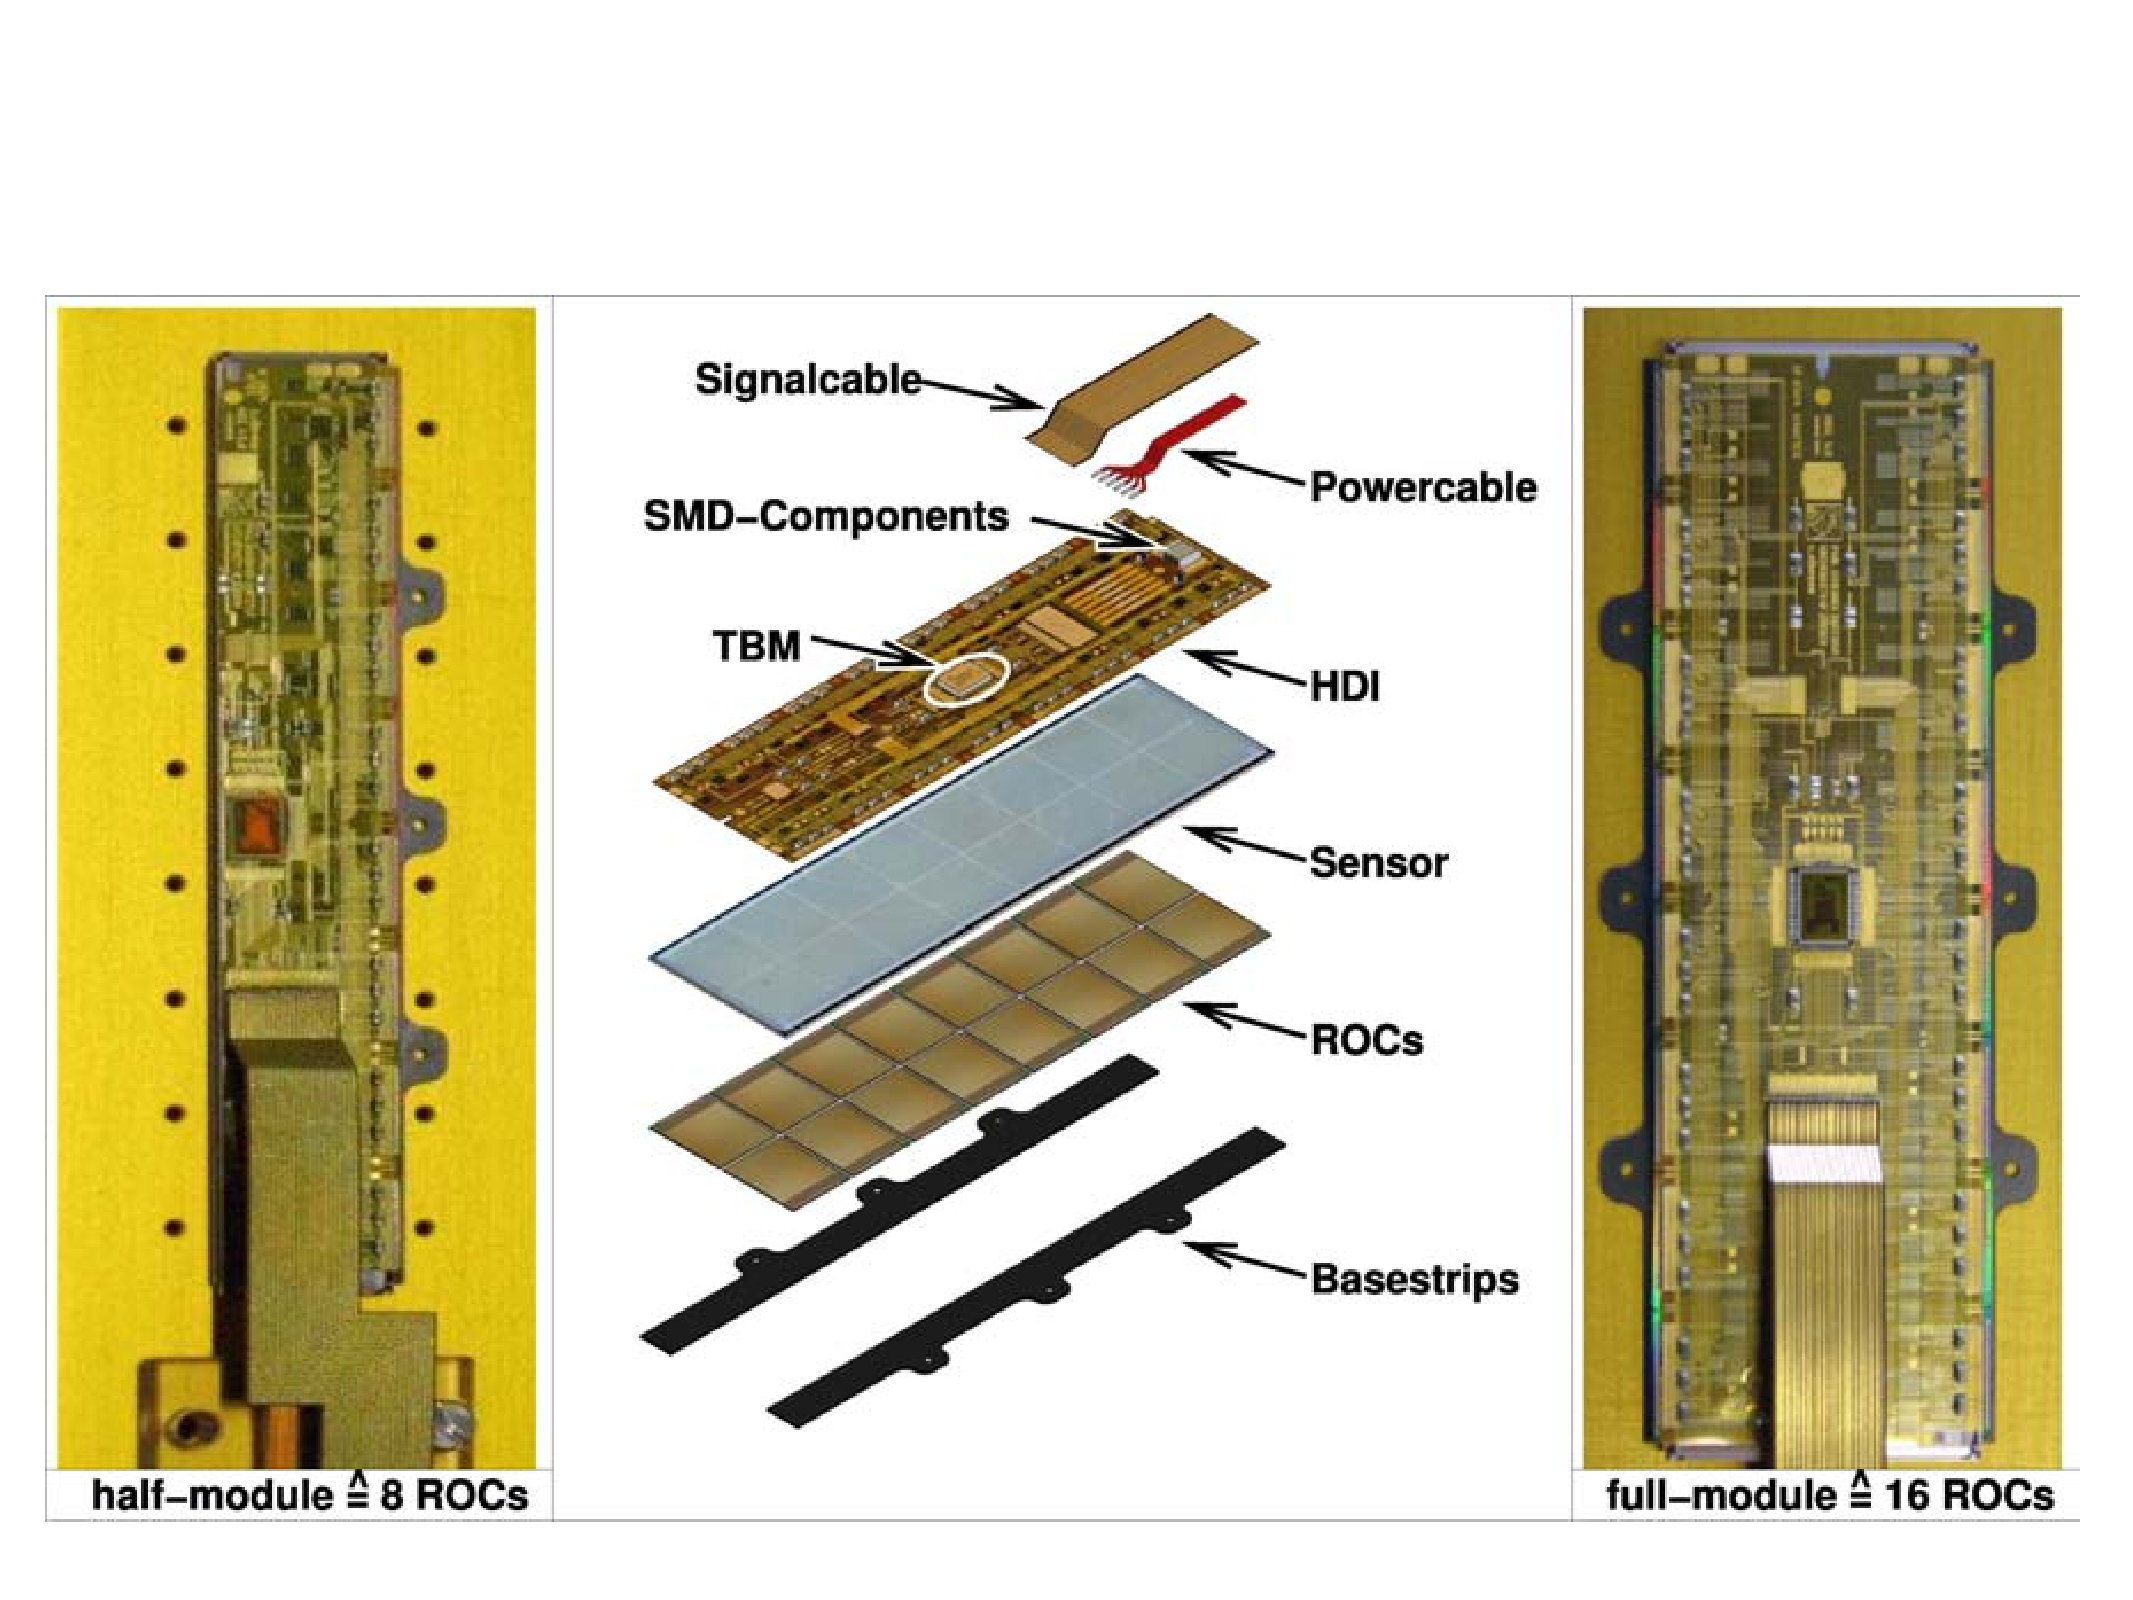
\includegraphics[width=0.99\textwidth]{CMS_DetectorFigures/BPixModule.pdf}
 \caption{BPix completed modules; (left) half-module, (center) an
   schematic of the different component forming the a full-module,(right) full-module.\label{fig:Bpix}}
\end{figure}
\begin{figure}
 \centering
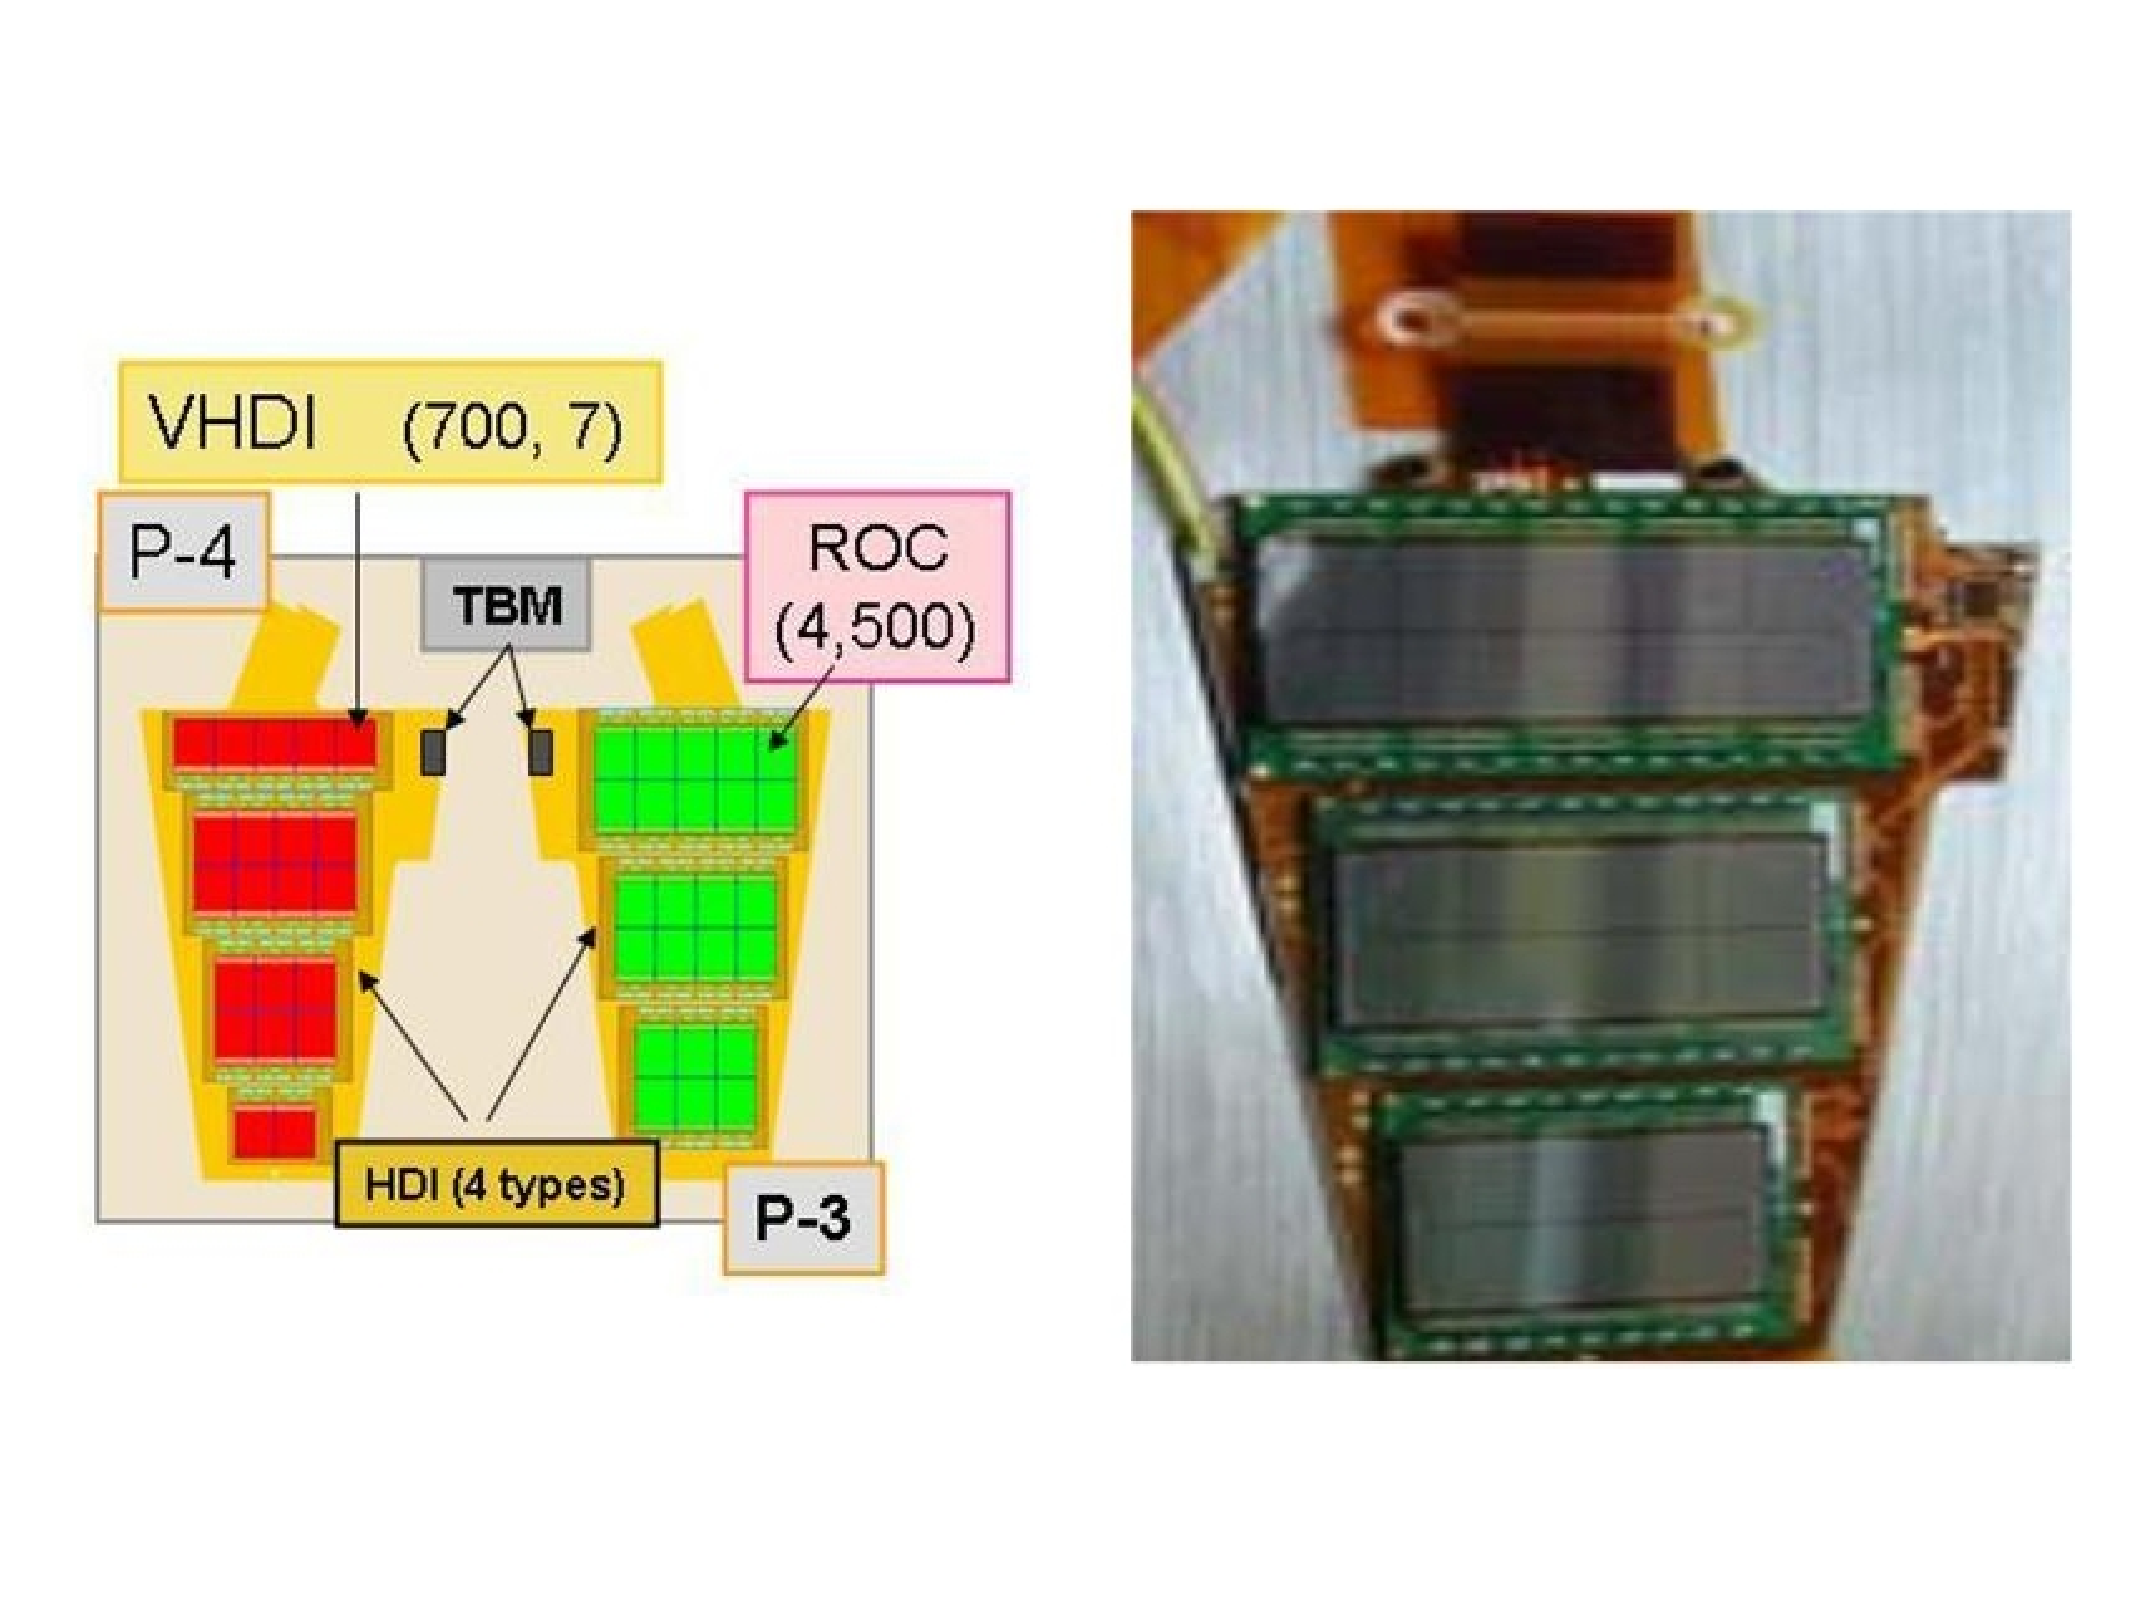
\includegraphics[width=0.99\textwidth]{CMS_DetectorFigures/FPixModule.pdf}
 \caption{FPix module; (left) an schematic of the two types of module,
   (right) a photograph of one of the completed FPix modules.\label{fig:Fpix}}
\end{figure}

\begin{figure}
 \centering
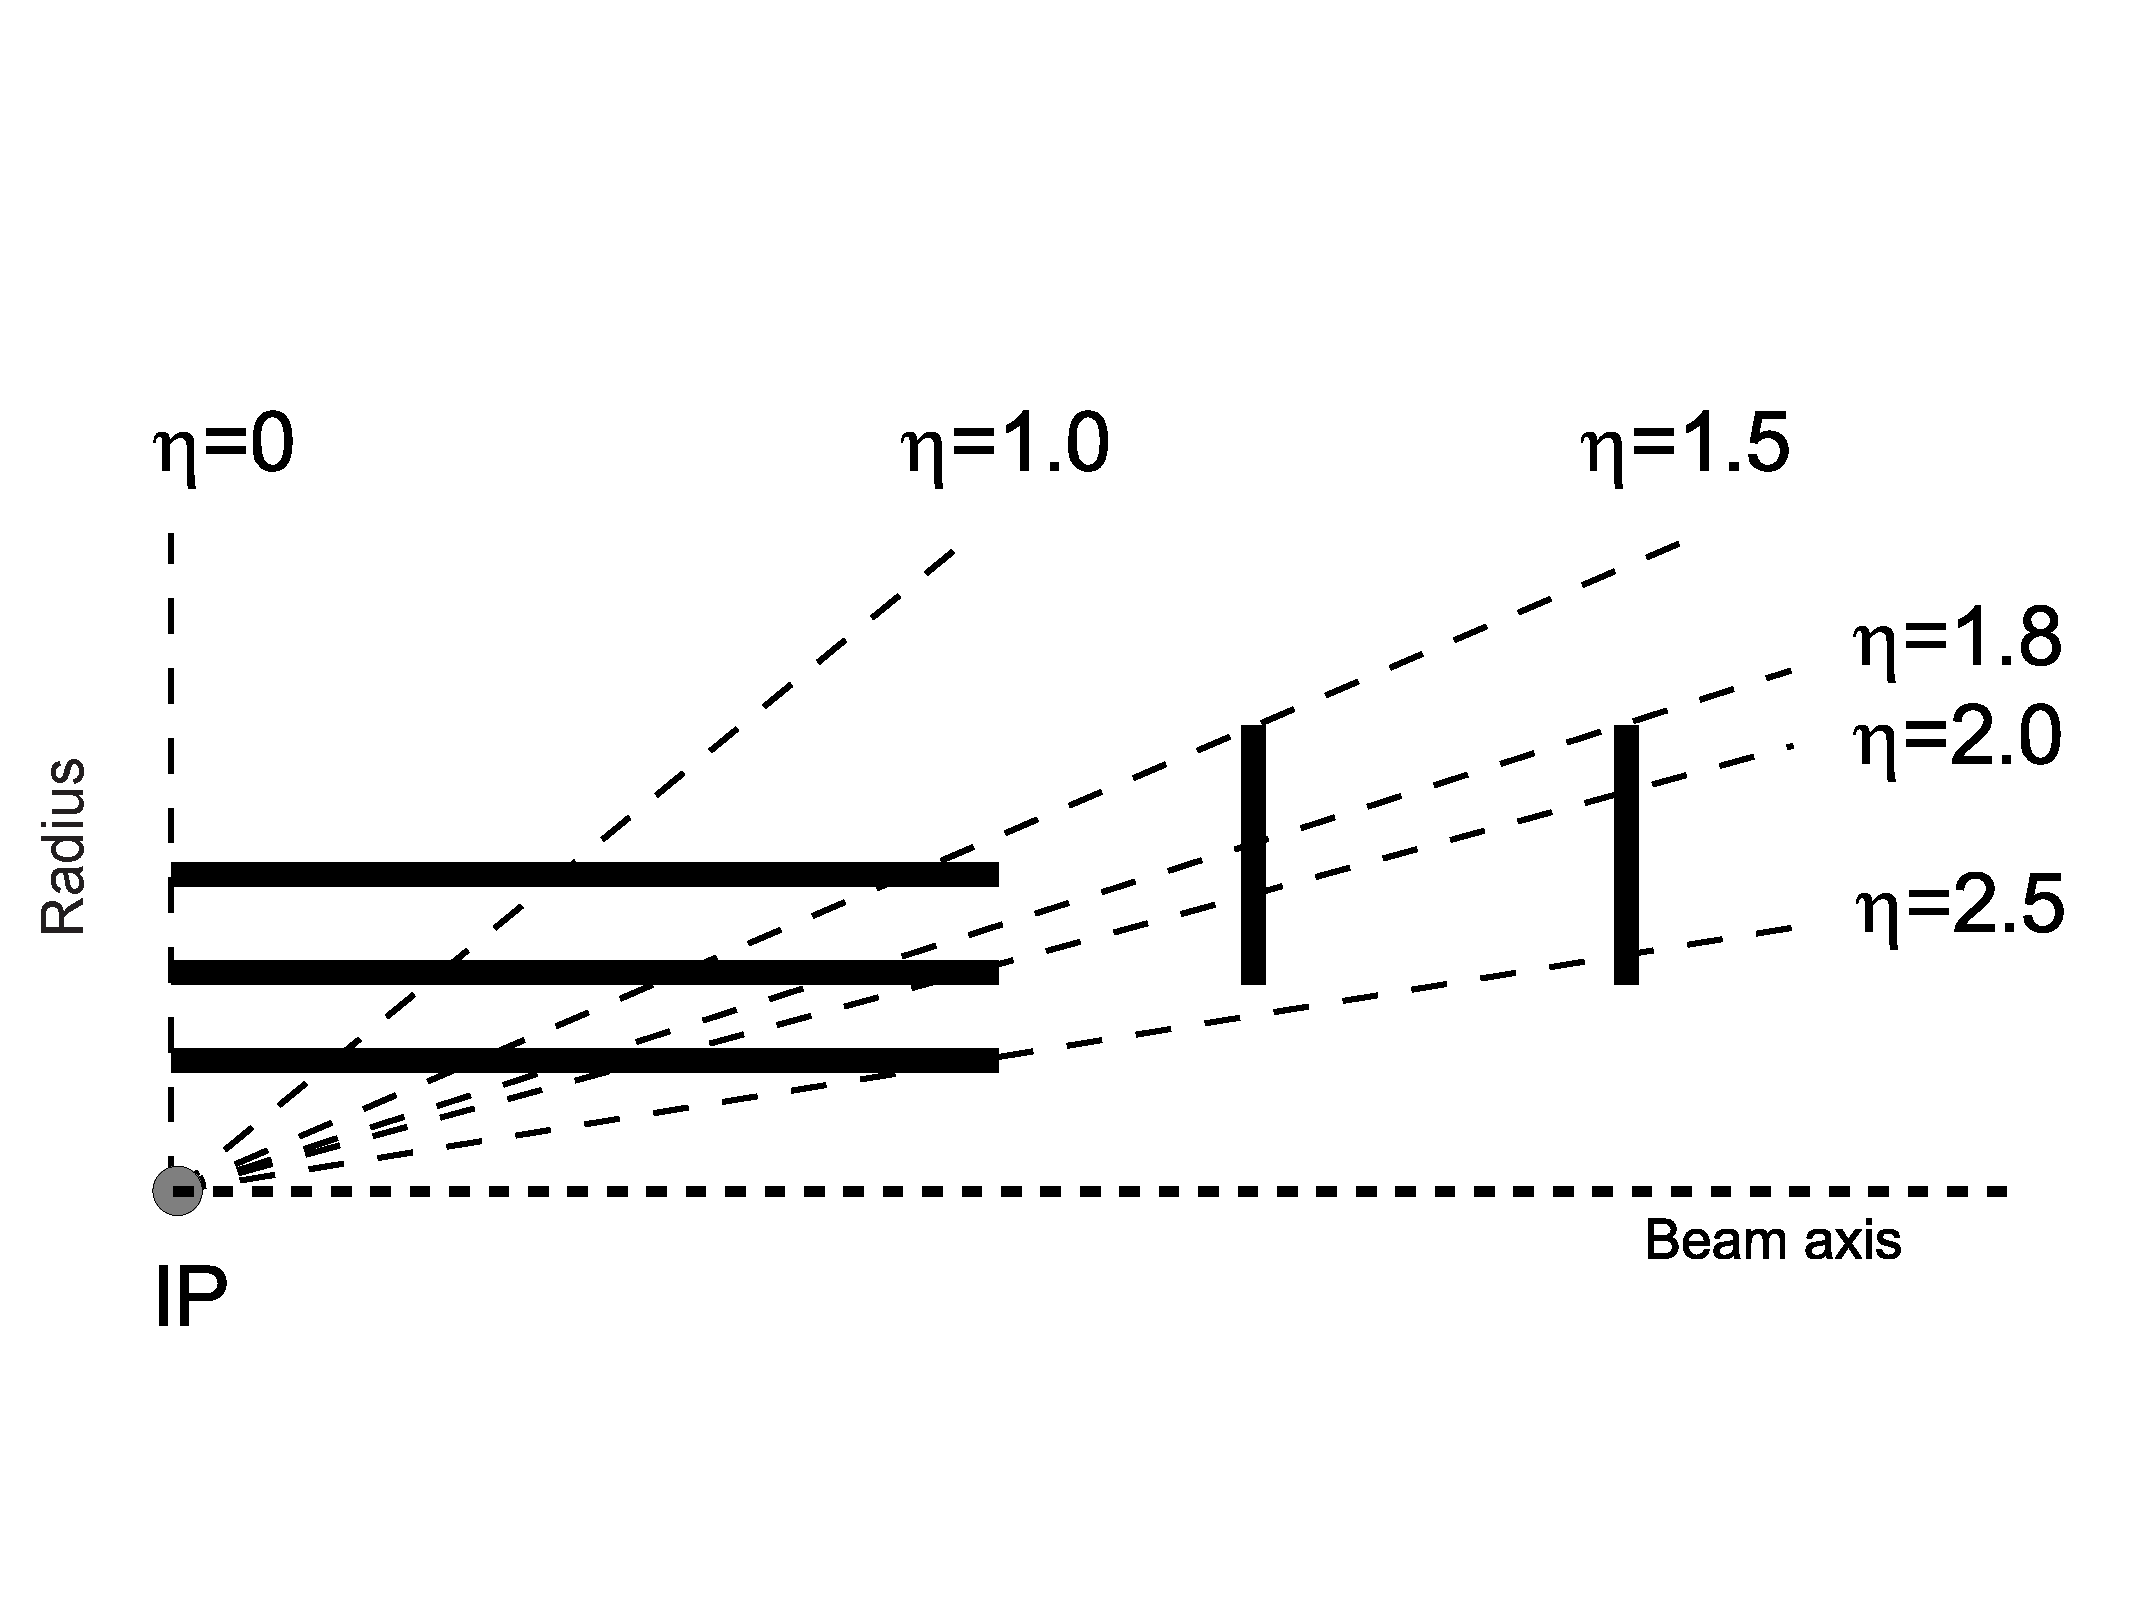
\includegraphics[width=0.49\textwidth]{CMS_DetectorFigures/PixelLayout.pdf}
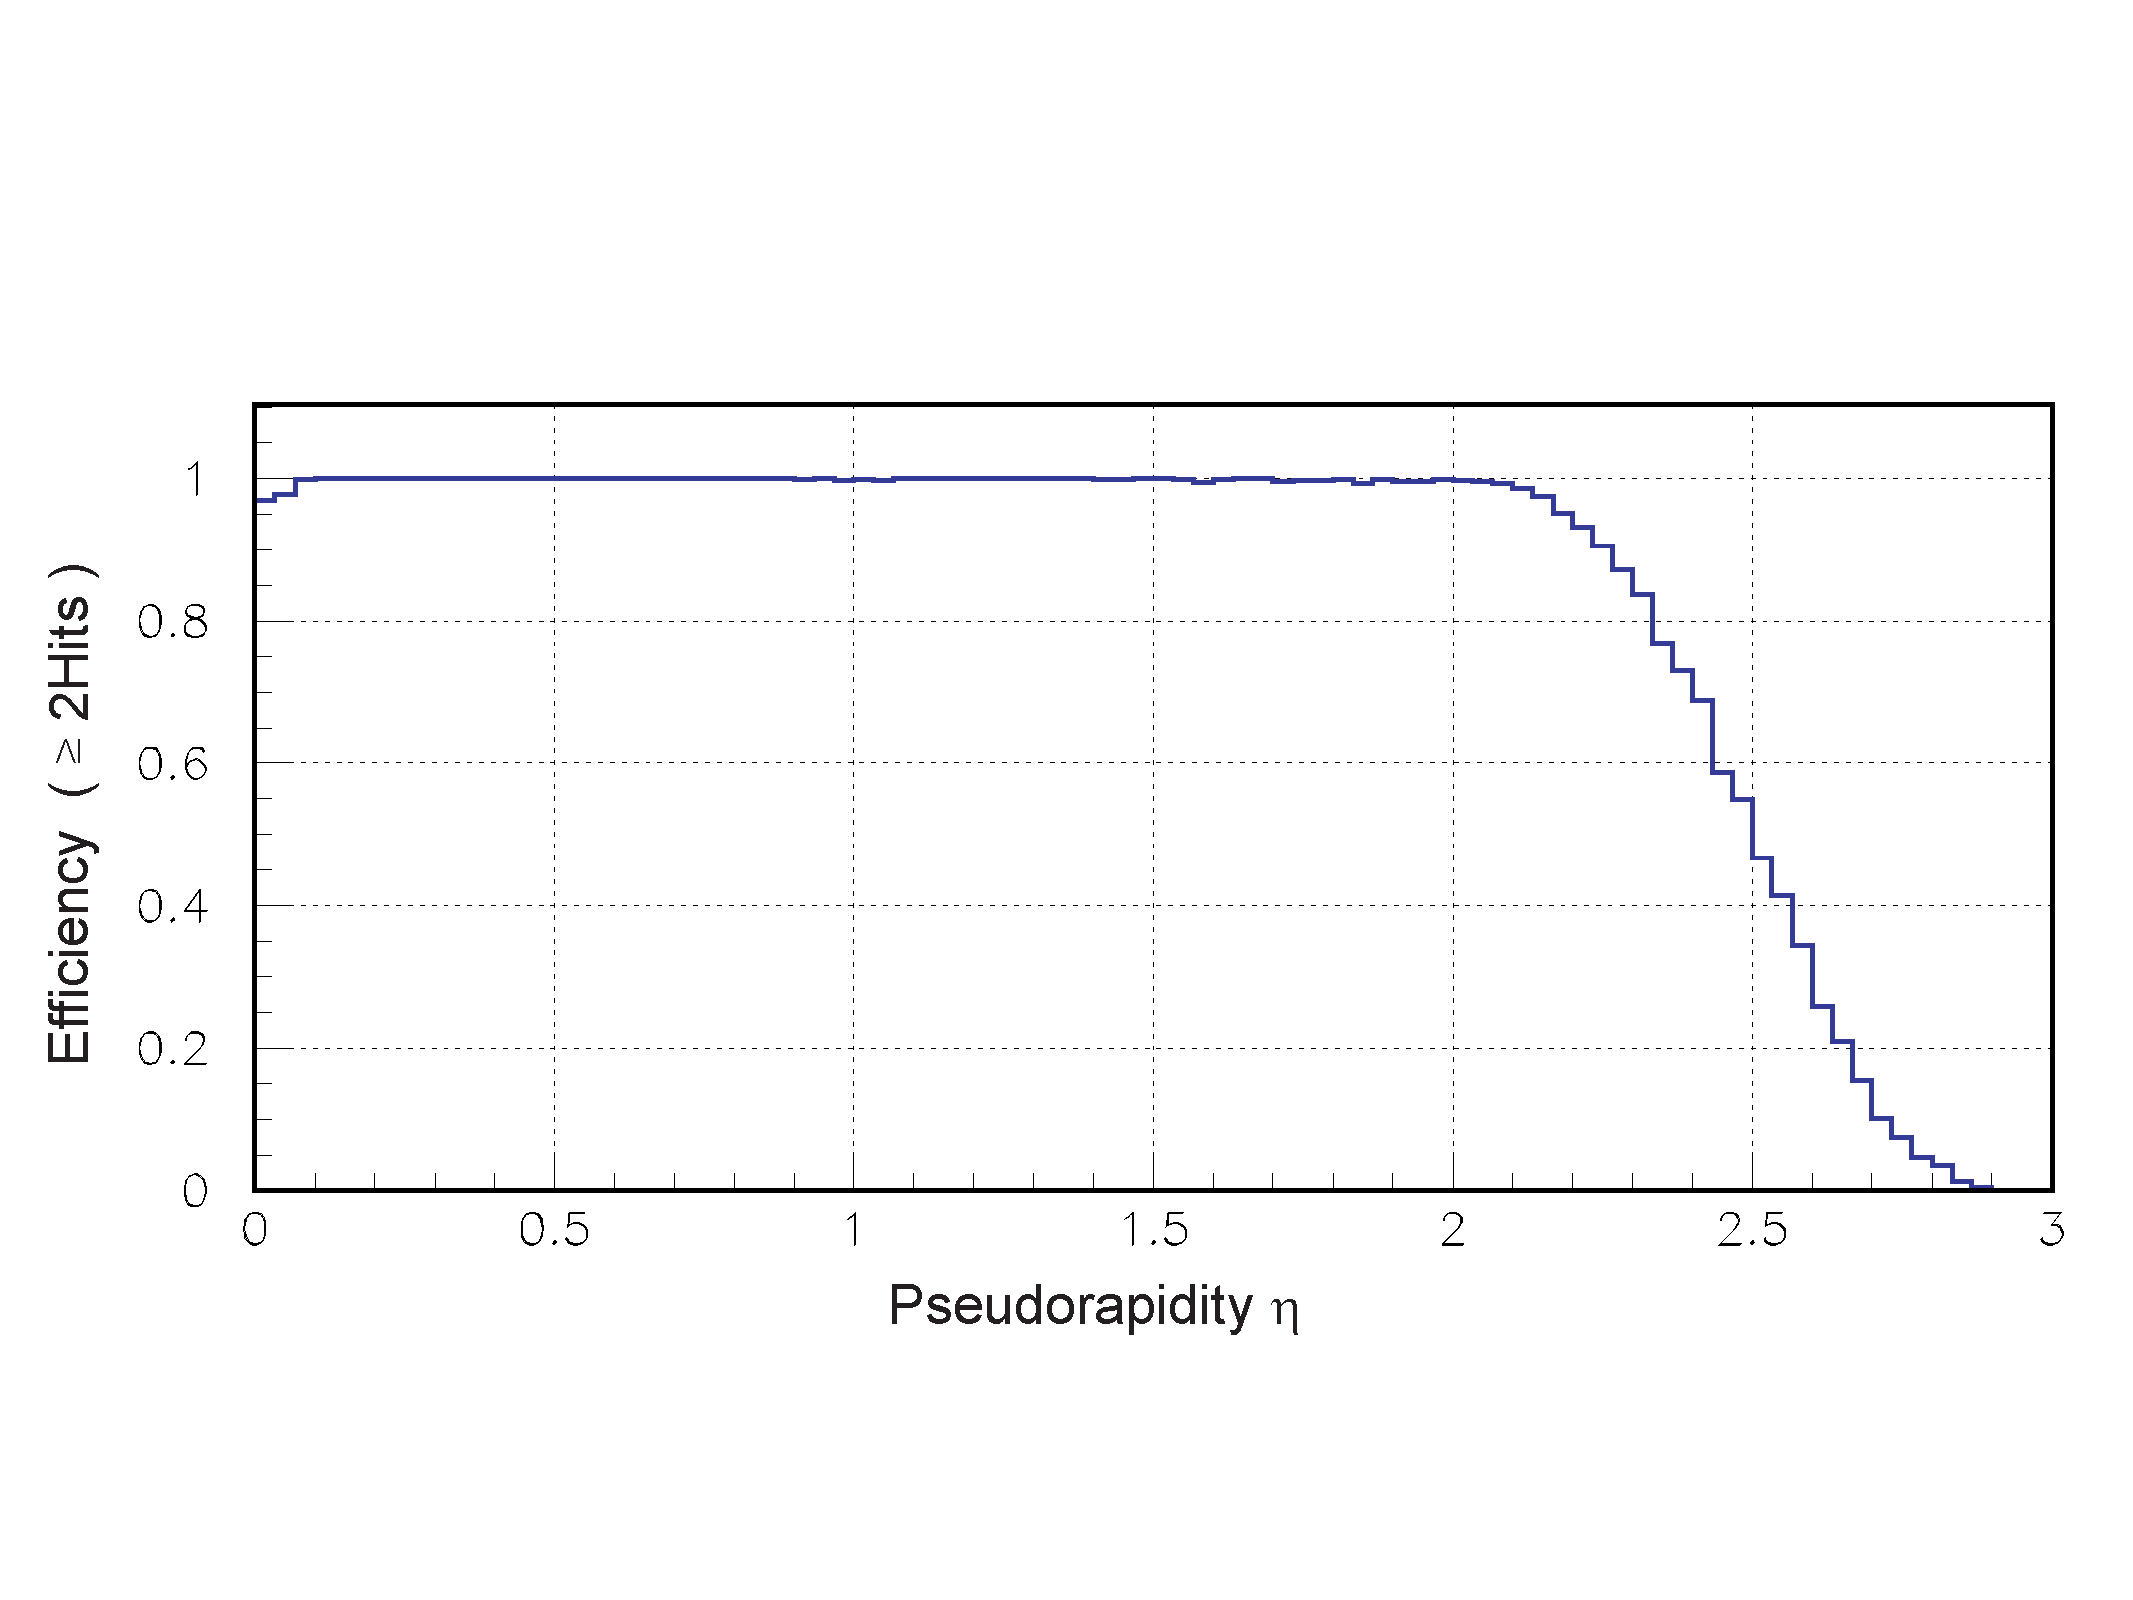
\includegraphics[width=0.49\textwidth]{CMS_DetectorFigures/PixelEfficiency.pdf}
 \caption{(Left) the layput of the silicon pixel tracker, (right) the
   pixel tracker detection efficiency as a function of the pseudorapidity.\label{fig:PixelLayout}}
\end{figure}
\subsection{Strip Tracker}
The silicon tracker is located outside the inner pixel tracker and is
composed of three subsystems that extend from 20 cm to 116 cm in the
radial direction. The Tracker Inner Barrel and Disks (TIB/TID) are
the innermost subsystem extending up to a radius of 55 cm, it includes
4 barrel layers and 3 disks at each side. The TIB/TID with their 320
$\mu$m thick silicon micro-strip sensor oriented along the $z$-axis records up to 4 $r$-$\phi$
measurements on a particle's trajectory. The strips pitch  in the TIB -- the
distance between each strip -- varies between 80 $\mu$m and 120 $\mu$m
in layers 1-2 and 3-4, respectively. The resulting single point
resolution is therefore 23 $\mu$m and 35 $\mu$m for the 1-2 and 3-4
layers, respectively. The TID has strip pitches between 100 -140$\mu$m
-- resulting in single point resolution between 29-41 $\mu$m. The
TIB/TID is completely sorrounded by the Tracker Outer Barrel (TOB)
which with its 6 barrel layer extends up to a radious of 116 cm. The
layers are composed of 500 $\mu$m thick micro-strips sensor with
pitches of 183 $\mu$m and 122 $\mu$m for the firts 4  and last 2
layer, respectively -- recording up to 6 $r$-$\phi$
measurements on a particle's trajectory with single point resolutions of 53 $\mu$m
and $\mu$m, respectively. The TIB/TID and the TOB cover the region
with $|z|< 113$ cm, beyond this point (see
Figure~\ref{fig:trackerlayout}) the Tracker EndCaps (TEC$^{\pm}$) --
where the sign, obiously, represents the position on the $z$-axis --
extend from 124 cm $|z|< 282$ cm and 22.5 cm $|r|< 113.5$ cm. The TEC
consists of 9 disks which contains up to 7 rings of silicon
micro-strips, the later are 320 $\mu$m and 500 $\mu$m thick in the
inner 4 and outer 3 rings, respectively.
Additionally, modules in the two innermost layers in the TIB and TOB,
the two inner most rings of the TID, as well as rings 1,2 and 5 of the TECs are
equipped with a second micro-strip detector module that is mounted
back-to-back allowing measurements on the perpedicular coordinate --
i.e. $z$ and r in the barrel and the disks, respectively. In this
fashion at least $\approx$ 9 hits in the silicon strip tracker in the
$|\eta|<2.4$ range are ensure, with at least $\approx$ 4
two-dimensional measurements. The full strip tracker amounts to a
total of 9.3 million strips and covers an active are of silicon equal
to 198 m$^2$.

\section{The Electromagnetic Calorimeter}
\section{The Hadronic Calorimeter}
\section{The Superconducting Solenoid}
\section{The Muon Chambers}